\pdfoutput=1
\documentclass[11pt]{article}

\usepackage[margin=1in]{geometry}
\usepackage{booktabs}
\usepackage{graphicx}
\usepackage{amsmath}
\usepackage{hyperref}
\usepackage[numbers]{natbib}

\title{nanoGenRec: An Agentic Research Framework for Landing Semantic-ID Generative Recommendation}

\author{
  Ziqing Ye \\
  \texttt{yeziqing986@gmail.com}
}

\date{\today}

\begin{document}

\maketitle

\begin{abstract}
AI agents can now read papers, write code, and launch experiments, but research progress still depends on a harder layer: maintaining a reproducible operating system around hypotheses, configs, long-running jobs, evaluation contracts, failed runs, and human decisions. We present \textsc{nanoGenRec}, an open-source agentic research framework that makes this layer explicit for Semantic-ID generative recommendation. The framework provides paper-note memory, role-neutral human-agent task exchange, YAML experiment configuration, duplicate-run detection, runtime estimation, queue-based execution, full-recall evaluation checks, decision records, and durable experiment logs. Its design is distilled from a real business research setting rather than a toy benchmark: coding, experiment execution, GPU scheduling, metric interpretation, and paper writing had to remain coherent while private data, long-running jobs, and changing research hypotheses were handled by agent-assisted workflows. The private empirical lineage contains 51 recorded experiments, behavior sweeps up to 7.85M users and 299.0M raw interactions, roughly 445M effective SID tokens after truncation, million-item SID caches, and experiments run in a real 4$\times$NVIDIA H200 GPU environment. Within this agent-managed workspace, the GR stack serves as a demanding validation target and produces traceable evidence of model scaling, non-monotonic behavior-window effects under temporal drift, tokenizer-capacity tradeoffs, SID-constrained retrieval, and post-training alignment failures caused by rollout distribution mismatch. The released artifact removes private data and deployment details while preserving the research machinery: configs, logs, validation checks, public notebooks, and reproducible code paths. A small MovieLens 1M Colab-T4 path is included only as a public execution proof that the same Qwen embedding $\rightarrow$ SID construction $\rightarrow$ NTP training $\rightarrow$ reward-alignment $\rightarrow$ full-evaluation loop can run without private data. We position \textsc{nanoGenRec} primarily as an agentic research workspace and landing record: a way for researchers and agents to turn complex recommender-system ideas into auditable, recoverable, executable research programs.
\end{abstract}

\section{Introduction}

Generative Recommendation (GR) is moving recommender systems from multi-stage retrieve-and-rank pipelines toward autoregressive generation over item tokens. Industrial reports such as OneRec~\citep{onerec}, OneRec-V2~\citep{onerecv2}, OneMall~\citep{onemall}, GenRec~\citep{genrec}, OneLive~\citep{onelive}, and GR4AD~\citep{gr4ad} show that Semantic-ID generation, model scaling, and preference alignment can be viable at production scale.

The public literature now contains strong system diagrams and deployment evidence, yet there is still a practical gap for researchers who want to turn those ideas into a running system. A working GR system needs more than a model definition. It needs a tokenizer that maps items into discrete semantic tokens, a behavior preprocessing path that produces autoregressive training sequences, a model and training loop, a constrained generation procedure that maps generated tokens back to items, a full-recall evaluation protocol, and experiment infrastructure that can distinguish real improvements from duplicated baselines, invalid feature plumbing, or inline-evaluation artifacts. In practice, the system either works end to end or the individual components are hard to interpret.

We introduce \textsc{nanoGenRec}, an open-source agentic research framework and empirical record for landing Semantic-ID-based generative recommendation. The project is built from production-grounded experiments in a real business research setting, with private data and deployment-specific details removed. Its purpose is not to claim a new recommendation algorithm. Instead, it shows how a research agent and human collaborator can assemble, execute, evaluate, debug, and iterate on a GR stack in a reproducible workspace. The accompanying experiment lineage records both positive results and failure modes, making the framework useful as a reference implementation, an operational checklist, and a durable research memory.

The claim boundary is explicit. \textsc{nanoGenRec} does not claim online production gains, a new tokenization algorithm, or a new preference-optimization objective. Its contribution is a landed research framework: the agent protocol, code paths, experiment contracts, evaluation protocol, and logs needed to make Semantic-ID GR run as a real retrieval system and to reproduce a set of useful GR behaviors under that framework.

This report makes five contributions:

\begin{enumerate}
  \item \textbf{An agentic research framework.} We release paper-note memory, role-neutral task exchange, status tracking, decision records, runtime estimation, YAML experiment configuration, duplicate-run checks, and queue-based long jobs for recommendation research.
  \item \textbf{A nontrivial GR validation target.} We instantiate the framework on an end-to-end Semantic-ID GR workflow covering tokenization, NTP training, reward alignment, SID-constrained beam search, and full-recall evaluation.
  \item \textbf{Agent-managed empirical lineage.} Within the same framework, we preserve model scaling, tokenizer-capacity effects, full-recall baselines, and post-training alignment dynamics as traceable experiment records rather than isolated result tables.
  \item \textbf{Production-grounded scale with public execution proof.} We report a seven-point NTP scaling sweep, a behavior-window study, tokenizer and embedding sweeps, full-eval baselines, and an off-policy/on-policy ECPO comparison from a private real-world lineage. A redistributable MovieLens 1M Colab-T4 run verifies that the released interfaces execute end to end.
  \item \textbf{Failure-aware reproducibility.} We preserve experiment logs for successes, negative results, invalid runs, and post-training collapses, including the conditions under which a GR experiment becomes invalid.
\end{enumerate}

\section{Background}

\subsection{Agentic Research Frameworks}

Recent agent frameworks show that LLM agents benefit from explicit interfaces, memory, and workflow structure. SWE-agent argues that agents are a distinct class of computer users and improves software-engineering performance through an agent-computer interface designed for repository navigation, editing, and testing~\citep{sweagent}. AutoGen provides a general infrastructure for composing conversable agents, tools, and human participation~\citep{autogen}. Voyager demonstrates that long-horizon agents can improve by accumulating executable skills and using environment feedback for self-verification~\citep{voyager}. Agent Laboratory organizes research assistance into literature review, experimentation, and report writing stages with human feedback~\citep{agentlaboratory}.

\textsc{nanoGenRec} is closest in spirit to this line of work, but targets a different bottleneck: durable research state for long-running empirical ML systems. The main object is not a single conversation pattern, a single software issue, or a final generated report. It is the repository state needed to keep a research program coherent across weeks of experiments: paper memory, human-agent instructions, YAML configs, duplicate-run checks, queues, full-evaluation contracts, invalid-run records, and phase-level summaries. This makes the framework closer to a research operating system than to a task agent.

\begin{table}[t]
\centering
\caption{Positioning of \textsc{nanoGenRec} relative to representative agent frameworks.}
\label{tab:agentic-positioning}
\small
\begin{tabular}{p{0.18\linewidth}p{0.32\linewidth}p{0.40\linewidth}}
\toprule
Framework & Primary abstraction & Difference in \textsc{nanoGenRec} \\
\midrule
SWE-agent & Agent-computer interface for code tasks & Repository-native research state for experiments, not only issue solving \\
AutoGen & Conversable multi-agent orchestration & Durable artifacts and eval contracts, not only agent conversation patterns \\
Voyager & Skill library with environment feedback & Experiment lineage and decision memory, not reusable game skills \\
Agent Laboratory & Research pipeline from idea to paper & Long-running empirical loop with queues, invalid runs, and full-eval governance \\
\textsc{nanoGenRec} & Agentic research operating system & GR is a stress-test workload for auditable empirical research \\
\bottomrule
\end{tabular}
\end{table}

This positioning also explains why GR is a useful validation workload. Generic coding agents can modify files, and generic multi-agent frameworks can route messages, but real empirical recommendation research fails at slower boundaries: a feature is written but not consumed by training, an inline metric is mistaken for full recall, a duplicated config consumes expensive GPU time, or an invalid run is forgotten and later reinterpreted as evidence. \textsc{nanoGenRec} therefore optimizes for iteration integrity rather than only task completion. Its artifacts make three properties explicit: \emph{what should be run}, \emph{whether it has already been run}, and \emph{whether the resulting number is valid under the evaluation contract}. These properties are especially important when the private workload is large enough that each mistake may cost multi-GPU time and delay multiple downstream decisions.

\subsection{Semantic-ID Generative Recommendation}

Semantic-ID GR represents each item as a short sequence of discrete tokens. Recommendation then becomes conditional generation: given a user's behavior history, a model predicts the token sequence of the next target item. This formulation allows recommendation to reuse autoregressive modeling, beam search, MoE scaling, and post-training alignment ideas from generative AI.

Recent industrial systems have explored this direction from complementary angles. OneRec introduced an end-to-end generative architecture and reported production deployment with scaling and reinforcement learning evidence~\citep{onerec}. OneRec-V2 improved scalability with a lazy decoder-only design and real-world preference alignment~\citep{onerecv2}. OneMall unified several e-commerce scenarios with Semantic Tokenization, Transformer-based generation, and RL alignment~\citep{onemall}. GenRec introduced page-wise NTP, token merging, and GRPO-SR for preference-oriented recommendation~\citep{genrec}. OneLive adapted the paradigm to live-streaming with dynamic tokenization and multi-objective alignment~\citep{onelive}. GR4AD studied production advertising with value-aware learning and dynamic beam serving~\citep{gr4ad}.

These papers establish that GR can work in large industrial systems. \textsc{nanoGenRec} addresses a different layer of the problem: the missing reproducible workspace between those system descriptions and a runnable research implementation. It therefore complements prior work by exposing the operational interfaces, experiment governance, and failure records needed to iterate on GR outside the original production stacks.

\subsection{Reproducibility Gap}

GR papers typically report architecture and production results, while the operational details needed for reproduction are scattered across preprocessing, training, evaluation, and experiment management. Several details are easy to miss:

\begin{itemize}
  \item Inline evaluation during training is often a health check, not a comparable full-recall metric.
  \item Feature ablations can become invalid when preprocessing stores a feature but training or inference does not consume it.
  \item Tokenizer proxy metrics can disagree unless collision, balance, and behavior-aware semantic-neighbor retention are tracked together.
  \item RL-style post-training can collapse when rollout candidates are sampled from a distribution that no longer matches the current policy.
\end{itemize}

\textsc{nanoGenRec} treats these details as first-class experimental artifacts.

\section{The nanoGenRec Framework}

\textsc{nanoGenRec} is organized around one practical goal: a researcher or research agent should be able to move from a paper idea to a runnable experiment, evaluate it with the right contract, and recover the reasoning behind the result weeks later. The framework is therefore centered on research state rather than only model code: hypotheses, paper notes, configs, run queues, validation checks, metrics, failures, and decisions are all first-class artifacts.

\subsection{Agentic Research Loop}

The repository includes paper notes, decision records, status files, and a lightweight task-exchange protocol. Earlier versions used an explicit inbox/outbox because coding agents and experiment-running agents were intentionally separated: one session modified code and maintained the paper, while another session managed long GPU jobs and experiment queues. This separation matched the operational reality of a private business research workflow, where coding, GPU execution, and result interpretation did not always happen in the same interactive context. In the current framework, the same contract can be implemented either as files such as an inbox/outbox or as forked agent sessions that share repository state. The important design choice is not the folder name, but the durable handoff: hypotheses, run requests, blockers, results, and decisions must survive outside transient chat history.

This makes the framework role-neutral. A human can write an instruction, a coding agent can convert it into code and configs, an experiment agent can launch and monitor jobs, and a later paper-writing agent can recover the evidence without relying on memory from any single session. The agent reads papers, proposes ideas, estimates runtime, writes configs, checks prior experiments, and records decisions. The contribution here is operational: the research process is made inspectable and recoverable rather than embedded in transient chat logs or shell history.

The loop is deliberately failure-aware. Duplicate experiments are surfaced before launch, long jobs are queued instead of chained, inline metrics are separated from reportable full evaluation, and invalid runs are documented rather than overwritten. This is the main abstraction of the project. Semantic-ID GR is the first demanding workload used to test whether that abstraction can survive a real multi-stage research problem.

Figure~\ref{fig:agentic-loop} shows the agentic control loop. Each transition is backed by a repository artifact rather than by transient chat context. The agent can therefore resume from durable state, while the human collaborator can audit what was proposed, what was run, what failed, and why a direction changed. This is the mechanism that made the private lineage practical: many experiments were slow enough to outlive a single interactive session, and many failures were boundary failures between tokenizer, training, evaluation, and alignment code.

\begin{figure}[t]
\centering
\fbox{\begin{minipage}{0.94\linewidth}
\small
\begin{center}
\begin{tabular}{c}
\textbf{Paper notes + experiment logs} \\
$\Downarrow$ \\
\textbf{Hypothesis / task handoff} \\
$\Downarrow$ \\
\textbf{YAML config + duplicate-run registry check} \\
$\Downarrow$ \\
\textbf{Queued training / evaluation job} \\
$\Downarrow$ \\
\textbf{Full-recall metrics + failure diagnostics} \\
$\Downarrow$ \\
\textbf{Decision record + status update} \\
$\Longrightarrow$ \quad next research iteration
\end{tabular}
\end{center}
\end{minipage}}
\caption{Agentic research loop implemented by \textsc{nanoGenRec}. The loop turns paper reading, experiment design, execution, evaluation, and decision logging into auditable repository state. The task handoff may be an inbox/outbox folder, a forked agent session, or another repository-native protocol.}
\label{fig:agentic-loop}
\end{figure}

Table~\ref{tab:agentic-artifacts} lists the agent-facing contracts. These artifacts are intentionally mundane: their role is to make research progress recoverable. For example, a YAML config records the exact variant, a registry hash prevents duplicate reruns, the queue state separates long jobs from interactive sessions, and phase README files keep the current best result visible without rereading every log.

\begin{table}[t]
\centering
\caption{Agentic framework artifacts and the research failure modes they address.}
\label{tab:agentic-artifacts}
\begin{tabular}{p{0.22\linewidth}p{0.35\linewidth}p{0.33\linewidth}}
\toprule
Artifact & Research contract & Failure mode addressed \\
\midrule
Task handoff & Human instructions and agent findings are explicit & Lost context across sessions or roles \\
Paper notes & Prior work is summarized into reusable local memory & Re-reading or misremembering papers \\
YAML configs & Experiments override only intended parameters & Hidden or drifting hyperparameters \\
Registry hashes & Similar historical runs are surfaced before launch & Duplicate expensive experiments \\
Queue state & Long jobs are monitored asynchronously & Brittle script chains and forgotten runs \\
Full-eval reports & Reported numbers use the same evaluation contract & Inline metric overclaiming \\
Decision records & Negative results and pivots are written down & Cherry-picking and stale conclusions \\
\bottomrule
\end{tabular}
\end{table}

The design was shaped by repeated failure modes in the experiment lineage. EXP-026 records a SID trie construction bug where beam search produced zero candidates and the GRPO loss stayed at zero; the value of the framework is that this becomes a documented invalid run rather than a silent negative result. EXP-044 and EXP-044B record timestamp plumbing failures in which a temporal feature existed in preprocessing but was not actually available to the training/evaluation path; this motivated the rule that new features must be validated from preprocessing through beam search before drawing conclusions. EXP-028 records an off-policy ECPO collapse that only became visible under full-recall evaluation, while EXP-029 records the on-policy recovery. These cases are difficult to manage with a prompt-only agent loop: they require persistent run metadata, code-path checks, and a shared interpretation layer. They motivate the framework's insistence on full-eval contracts, explicit feature plumbing checks, and decision records.

\subsection{GR Stress-Test Pipeline}

The GR validation target consists of six stages:

\begin{enumerate}
  \item \textbf{Item representation.} Items are embedded with pretrained representation models. The current experiments use Qwen3 embeddings at several scales.
  \item \textbf{Semantic ID tokenization.} Embeddings are discretized into 3-token item IDs using residual KMeans and FSQ-family variants.
  \item \textbf{NTP preprocessing.} User behavior logs are converted into autoregressive training shards, with explicit date windows and evaluation targets.
  \item \textbf{Generative recommendation.} A Transformer+MoE NTP model predicts item SID tokens from user histories.
  \item \textbf{Full-recall evaluation.} SID-constrained beam search generates candidate item IDs, and Recall@K is computed with $K\in\{10,50,100,500\}$.
  \item \textbf{Experiment governance.} YAML configs, registry hashes, duplicate-run checks, queue-based execution, and phase-level README files preserve experiment lineage.
\end{enumerate}

Table~\ref{tab:framework-artifact} summarizes the combined agentic framework and GR validation target as a set of landing checks rather than only software modules.

\begin{table}[t]
\centering
\caption{Framework components and the landing checks they make reproducible.}
\label{tab:framework-artifact}
\begin{tabular}{p{0.20\linewidth}p{0.35\linewidth}p{0.35\linewidth}}
\toprule
Component & Landing check & Artifact produced \\
\midrule
SID tokenizer & Items map to valid multi-token IDs & SID cache and tokenizer metrics \\
NTP preprocessing & Behavior logs become training/eval shards & Date-bound shard configs \\
Transformer+MoE NTP & Histories predict next-item SID tokens & Checkpoints and train metadata \\
Constrained decoding & Generated tokens map back to real items & Full-recall candidate lists \\
Evaluation & Metrics use generated item IDs & Recall@K reports \\
Experiment runner & Runs are reproducible and deduplicated & YAML configs and registry hashes \\
Experiment logs & Results and failures are auditable & EXP notes and phase READMEs \\
\bottomrule
\end{tabular}
\end{table}

Table~\ref{tab:stage-parameters} makes the parameter level of each stage explicit. The production-scale empirical line and the public MovieLens line share the same framework interfaces, but they intentionally use different representation and model budgets.

\begin{table}[t]
\centering
\caption{Stage-level parameterization used by the production empirical study and the public Colab reproduction path.}
\label{tab:stage-parameters}
\begin{tabular}{p{0.20\linewidth}p{0.35\linewidth}p{0.35\linewidth}}
\toprule
Stage & Production empirical setting & Public MovieLens 1M setting \\
\midrule
Item representation & Qwen3 0.6B / 4B embeddings & Qwen3-Embedding-0.6B over public MovieLens metadata \\
SID tokenization & 3-token RKMeans/FSQ, 4096/8192 codebooks & residual KMeans, 16--64 clusters per layer \\
Sequence construction & 7--90 day windows, up to 445M SID tokens & Public ratings, max 100 items/user, sliding prefixes \\
NTP model & S/M/L tiers: 17.5M / 71.6M / 101.1M active params & Dense NTP, 2--3 layers, embed\_dim=96--128 \\
Training & YAML variants, queued multi-GPU production runs & 5--8 epochs, single Colab T4 \\
Alignment & SP-DPO / RF-DPO / GRPO / ECPO & Lightweight GRPO-style exact-SID reward stage \\
Evaluation & Full SID-constrained recall, R@10/R@500 & Beam=1000, 1,000 eval samples, R@1--R@1000 \\
Governance & Duplicate-run checks, EXP logs, phase READMEs & Notebook, metrics, public result page \\
\bottomrule
\end{tabular}
\end{table}

Figure~\ref{fig:shared-interface} shows the same point as a release diagram: the production line and the public MovieLens line differ in data and representation budget, but meet at the same framework interfaces.

\begin{figure}[t]
\centering
\fbox{\begin{minipage}{0.92\linewidth}
\small
\textbf{Production path:} Qwen3 item embeddings $\rightarrow$ RKMeans/FSQ SIDs $\rightarrow$ NTP shards $\rightarrow$ Transformer+MoE $\rightarrow$ preference/RL alignment $\rightarrow$ constrained full recall $\rightarrow$ EXP logs \\
\vspace{0.4em}
\textbf{Public path:} MovieLens metadata $\rightarrow$ Qwen3 item embeddings $\rightarrow$ residual KMeans SIDs $\rightarrow$ sliding-prefix shards $\rightarrow$ dense NTP $\rightarrow$ GRPO-style alignment $\rightarrow$ constrained full recall $\rightarrow$ public metrics \\
\vspace{0.4em}
\textbf{Shared interface:} item IDs $\leftrightarrow$ SID tokens, autoregressive SID sequences, valid-SID decoding, item-level Recall@K, and auditable run artifacts.
\end{minipage}}
\caption{Production and public paths share the same framework interfaces while using different data and representation budgets.}
\label{fig:shared-interface}
\end{figure}

\subsection{Experiment Orchestration}

New experiments inherit from a shared YAML base config and override only the parameters being tested. Multi-variant experiments are represented as a variant list. A registry hash excludes runtime paths and environment keys, allowing the runner to surface identical or near-identical historical runs before launching a new job. Queue-friendly wrappers support long-running training and evaluation without turning experiment scripts into brittle chains. Each completed run updates a local record of the hypothesis, design, metrics, and interpretation, so the repository accumulates a recoverable experiment lineage rather than only final checkpoints.

\subsection{Landing Criteria}

We treat GR as landed only when four criteria are met. First, generated token sequences must map back to real item IDs through the tokenizer vocabulary. Second, evaluation must use SID-constrained generation over the item space rather than an inline training proxy. Third, experiment changes must be reproducible from configs and traceable to logs. Fourth, failed runs must be diagnosable from recorded metrics and code-path checks. The empirical study below is organized around these criteria: model scaling tests whether the NTP core works, tokenizer sweeps test whether the item representation is usable, full-recall baselines test whether generation retrieves real items, and post-training experiments test whether alignment remains stable after the SFT stage.

\section{Experimental Setup}

\subsection{Data}

The empirical study uses anonymized production behavior data. The largest behavior sweep covers up to 7.85M users and 299.0M raw interactions. After sequence truncation, this corresponds to roughly 445M effective SID tokens. Private data and deployment-specific details are not released; the open-source artifact preserves the code, configs, evaluation protocol, and experiment logs. The main private logs still expose quantitative run scale: for example, the EXP-015 scaling run records 3,042,069 training sequences, 49,575 evaluation targets, 148,533 evaluation positions, 49,383 evaluation items, and 1,000 full-recall samples.

For public reproducibility, the repository also includes a compact MovieLens path. It uses public ratings and metadata to exercise the same interfaces: Qwen3 item representation, residual KMeans SID construction, sliding-prefix NTP training, a lightweight reward-alignment stage, constrained decoding, and item-recall evaluation. This path is intentionally treated as an execution proof for the released framework, while the main empirical evidence comes from the private real-world lineage described above.

\subsection{Compute}

The production-scale empirical experiments were run in a real 4$\times$NVIDIA H200 GPU environment. This hardware note is included to make the engineering scale of the experiment lineage interpretable; the released code does not depend on that environment. The public MovieLens proof run was executed on a single free Colab T4 GPU.

\subsection{Model Tiers}

We use three NTP model tiers, summarized in Table~\ref{tab:tiers}. Active parameters count only the routed compute used by each token.

\begin{table}[t]
\centering
\caption{NTP model tiers used in the empirical study.}
\label{tab:tiers}
\begin{tabular}{lrrrr}
\toprule
Tier & Embed Dim & Layers & Experts & Active Params \\
\midrule
S-tier & 256 & 6 & 8 & $\sim$17.5M \\
M-tier & 512 & 8 & 8 & $\sim$71.6M \\
L-tier & 512 & 12 & 16 & $\sim$101.1M \\
\bottomrule
\end{tabular}
\end{table}

\subsection{Evaluation Protocol}

Full evaluation uses SID-constrained beam search and reports item recall at several cutoffs. Unless otherwise stated, reported R@K values refer to full evaluation rather than inline training evaluation. This distinction matters because inline evaluation uses a limited candidate set and is intended for training health checks.

\section{Framework Validation and Empirical Study}

\textsc{nanoGenRec} validates the framework by asking whether the complete loop can reproduce behaviors that matter for GR practitioners. The following sections are therefore not independent benchmark claims. They are evidence that the same framework can support model scaling analysis, data-window analysis, tokenizer diagnosis, full-recall retrieval, and post-training alignment debugging.

\subsection{NTP Model Scaling}

The first validation target is the NTP core. If the framework has correctly connected SID tokenization, sequence construction, training, and evaluation, model scaling should produce a coherent curve rather than isolated wins. We trained seven model sizes from 1.7M to 101.1M active parameters on a fixed 262M-token dataset built from 31 days of behavior. The corresponding train metadata records 3,042,069 training sequences and 49,575 evaluation targets. Table~\ref{tab:model-scaling} reports the results.

\begin{table}[t]
\centering
\caption{NTP model scaling on a fixed 262M-token dataset.}
\label{tab:model-scaling}
\begin{tabular}{lrrrrr}
\toprule
Config & Active Params & PPL & Loss & R@10 & R@500 \\
\midrule
scale-01 & 1.7M & 235.1 & 5.460 & 1.9\% & 23.6\% \\
scale-02 & 3.6M & 100.4 & 4.609 & 3.7\% & 31.7\% \\
scale-03 & 5.1M & 69.6 & 4.243 & 5.4\% & 45.6\% \\
scale-04 & 17.5M & 28.1 & 3.334 & 9.8\% & 60.5\% \\
scale-05 & 34.5M & 24.0 & 3.178 & 11.5\% & 62.5\% \\
scale-06 & 71.6M & 20.8 & 3.037 & 12.6\% & 66.2\% \\
scale-07 & 101.1M & 19.4 & 2.965 & 13.7\% & 65.8\% \\
\bottomrule
\end{tabular}
\end{table}

The fitted loss curve is:

\begin{equation}
L(N) = 2.522 + \frac{2055.1}{N^{0.456}}.
\end{equation}

The exponent is close to the 0.489 exponent reported by OneRec-V2~\citep{onerecv2}. This is an important framework-level signal: the local implementation reproduces a recognizable GR scaling behavior while preserving full-recall metrics. Recall improves substantially through the S-tier and M-tier regime, while gains flatten between 71.6M and 101.1M active parameters under the fixed data budget. Figure~\ref{fig:scaling} shows the fitted curve.

\begin{figure}[t]
\centering
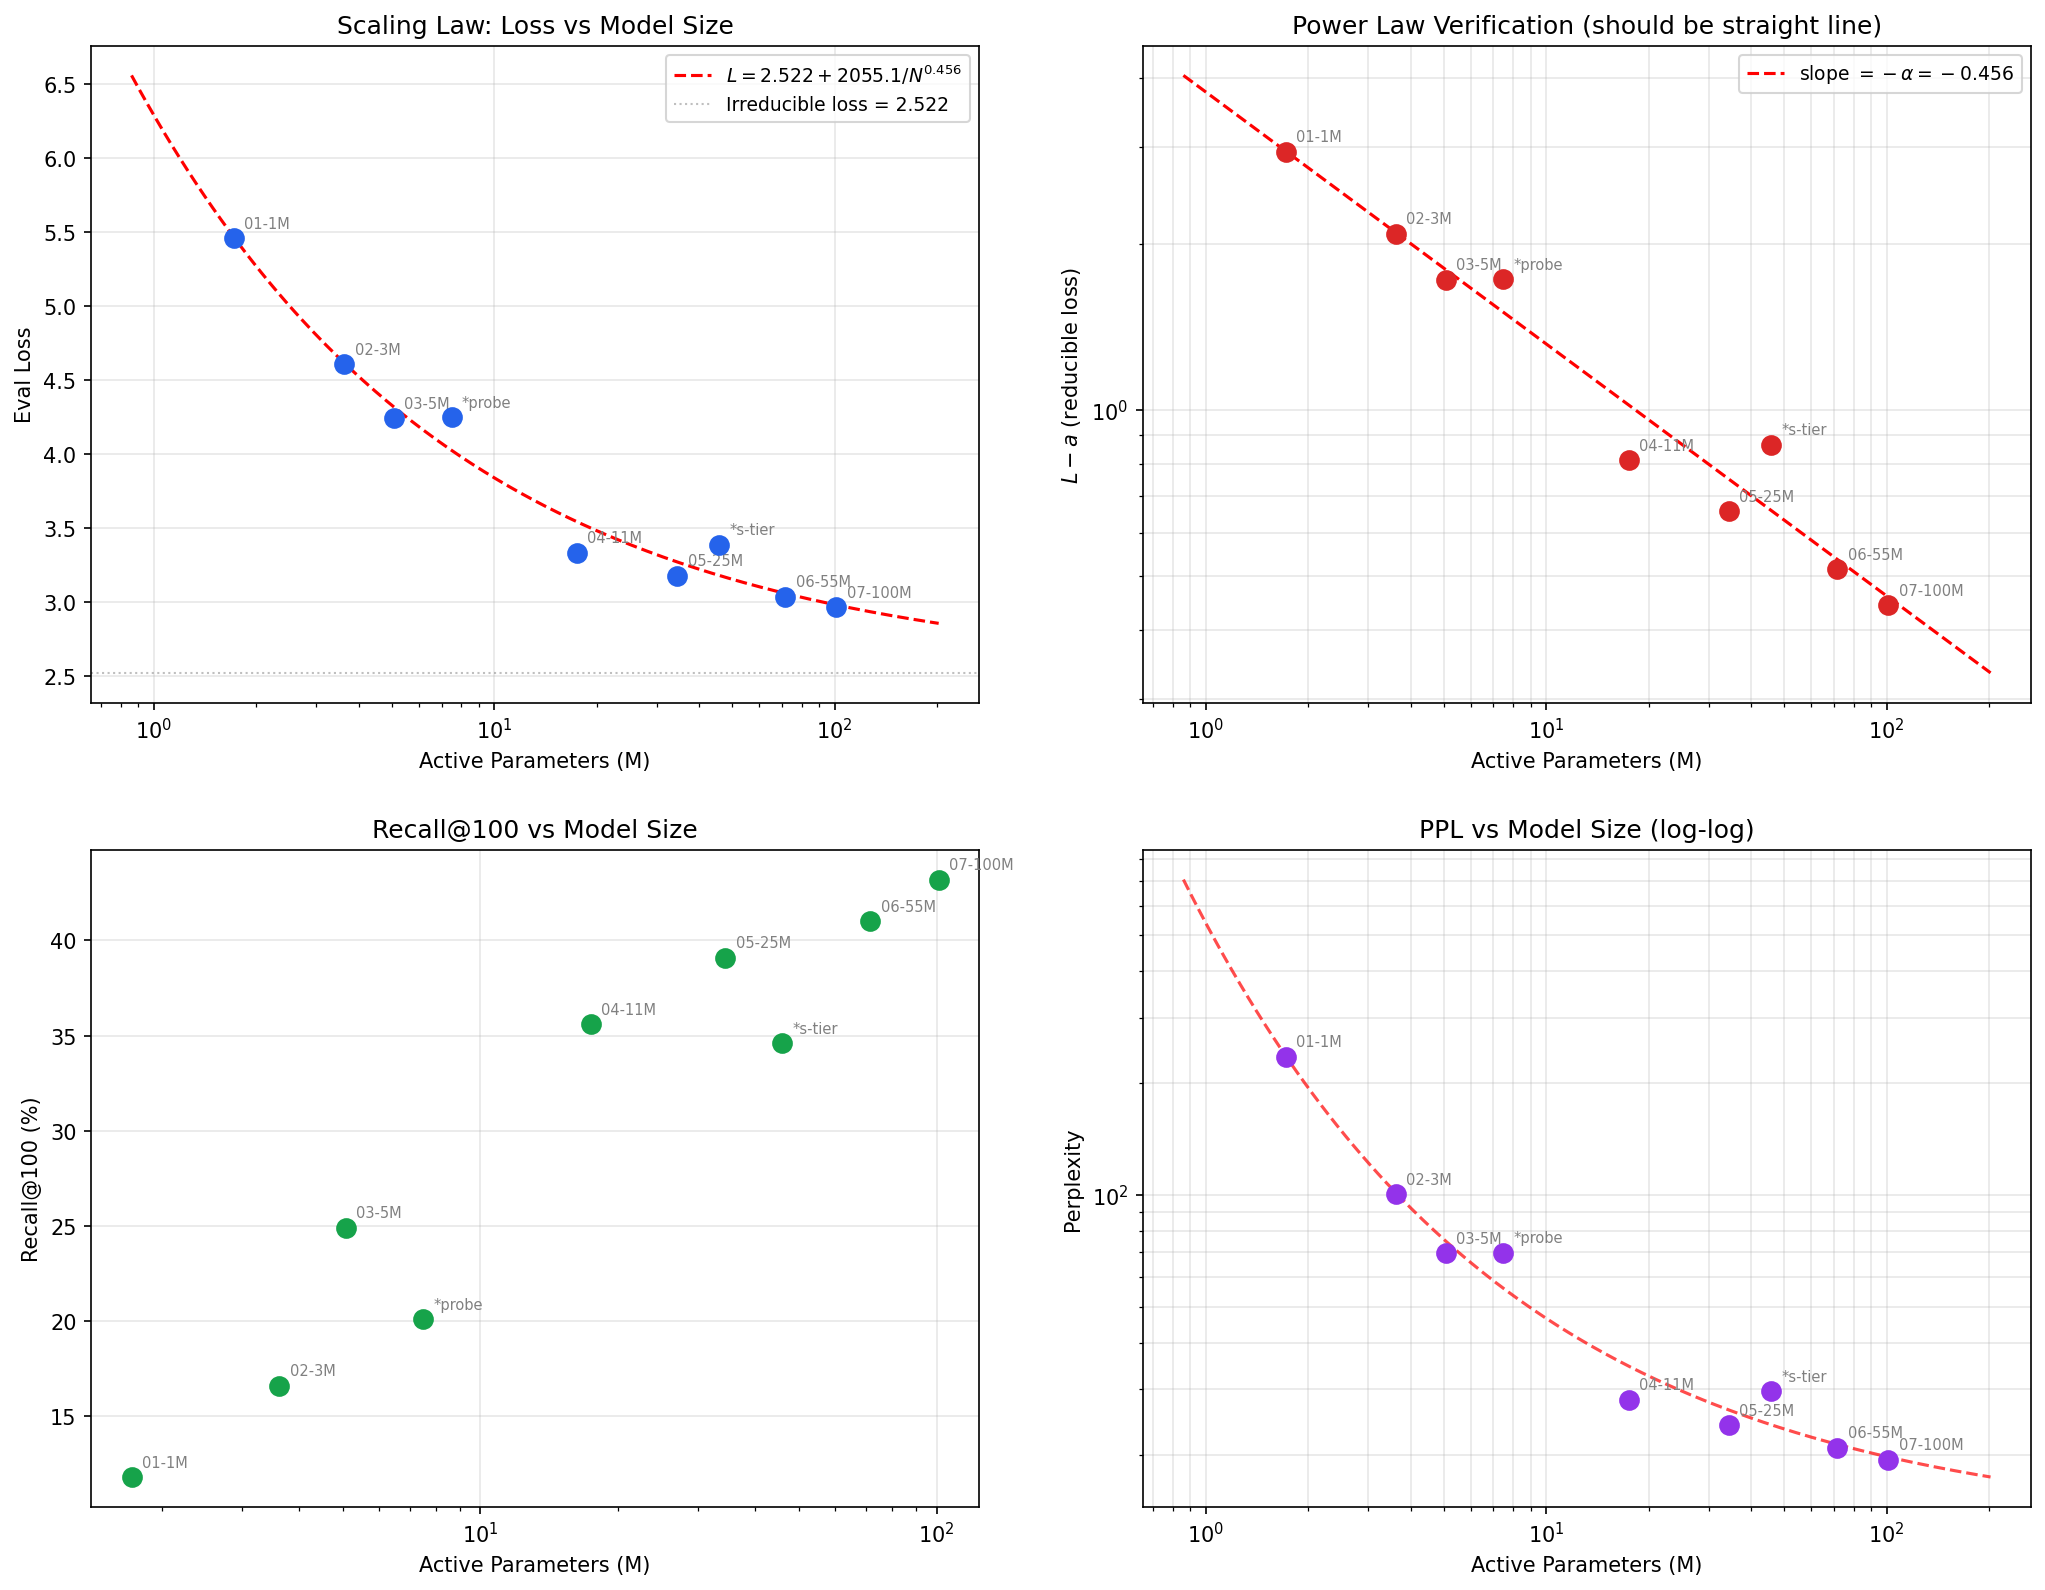
\includegraphics[width=0.78\linewidth]{figures/exp015-scaling-law.png}
\caption{NTP scaling law over active parameters.}
\label{fig:scaling}
\end{figure}

\subsection{Behavior-Window Scaling}

The second validation target is data plumbing under production time. We fixed the model tier and varied the behavior window. Standard compute-optimal scaling intuition~\citep{hoffmann2022chinchilla} suggests that more data should reduce loss under an i.i.d. assumption. Production recommendation behavior does not satisfy this assumption. Table~\ref{tab:data-scaling} summarizes the S-tier and M-tier data sweep.

\begin{table}[t]
\centering
\caption{Behavior-window scaling. The best loss occurs at 14 days, not at the longest window.}
\label{tab:data-scaling}
\begin{tabular}{lrrrrr}
\toprule
Config & Days & Tokens & Users & PPL & R@500 \\
\midrule
A-7d-S & 7 & 65M & 1.02M & 30.60 & 62.1\% \\
B-14d-S & 14 & 130M & 1.69M & 27.05 & 58.5\% \\
C-31d-S & 31 & 262M & 3.04M & 28.05 & 60.5\% \\
D-62d-S & 62 & 441M & 4.86M & 30.03 & 58.6\% \\
E-90d-S & 90 & 553M & 6.18M & 31.89 & 56.2\% \\
\midrule
A-7d-M & 7 & 65M & 1.02M & 19.31 & 70.7\% \\
B-14d-M & 14 & 130M & 1.69M & 18.96 & 65.8\% \\
C-31d-M & 31 & 262M & 3.04M & 19.39 & 65.8\% \\
D-62d-M & 62 & 441M & 4.86M & 19.80 & 68.1\% \\
\bottomrule
\end{tabular}
\end{table}

The main observation is non-monotonicity. Extending the window increases the number of users more than the per-user sequence depth, while older behavior can drift away from the current item pool. In this dataset, the exposure window is short enough that old behavior can become stale. Figure~\ref{fig:data-scaling} visualizes the effect.

\begin{figure}[t]
\centering
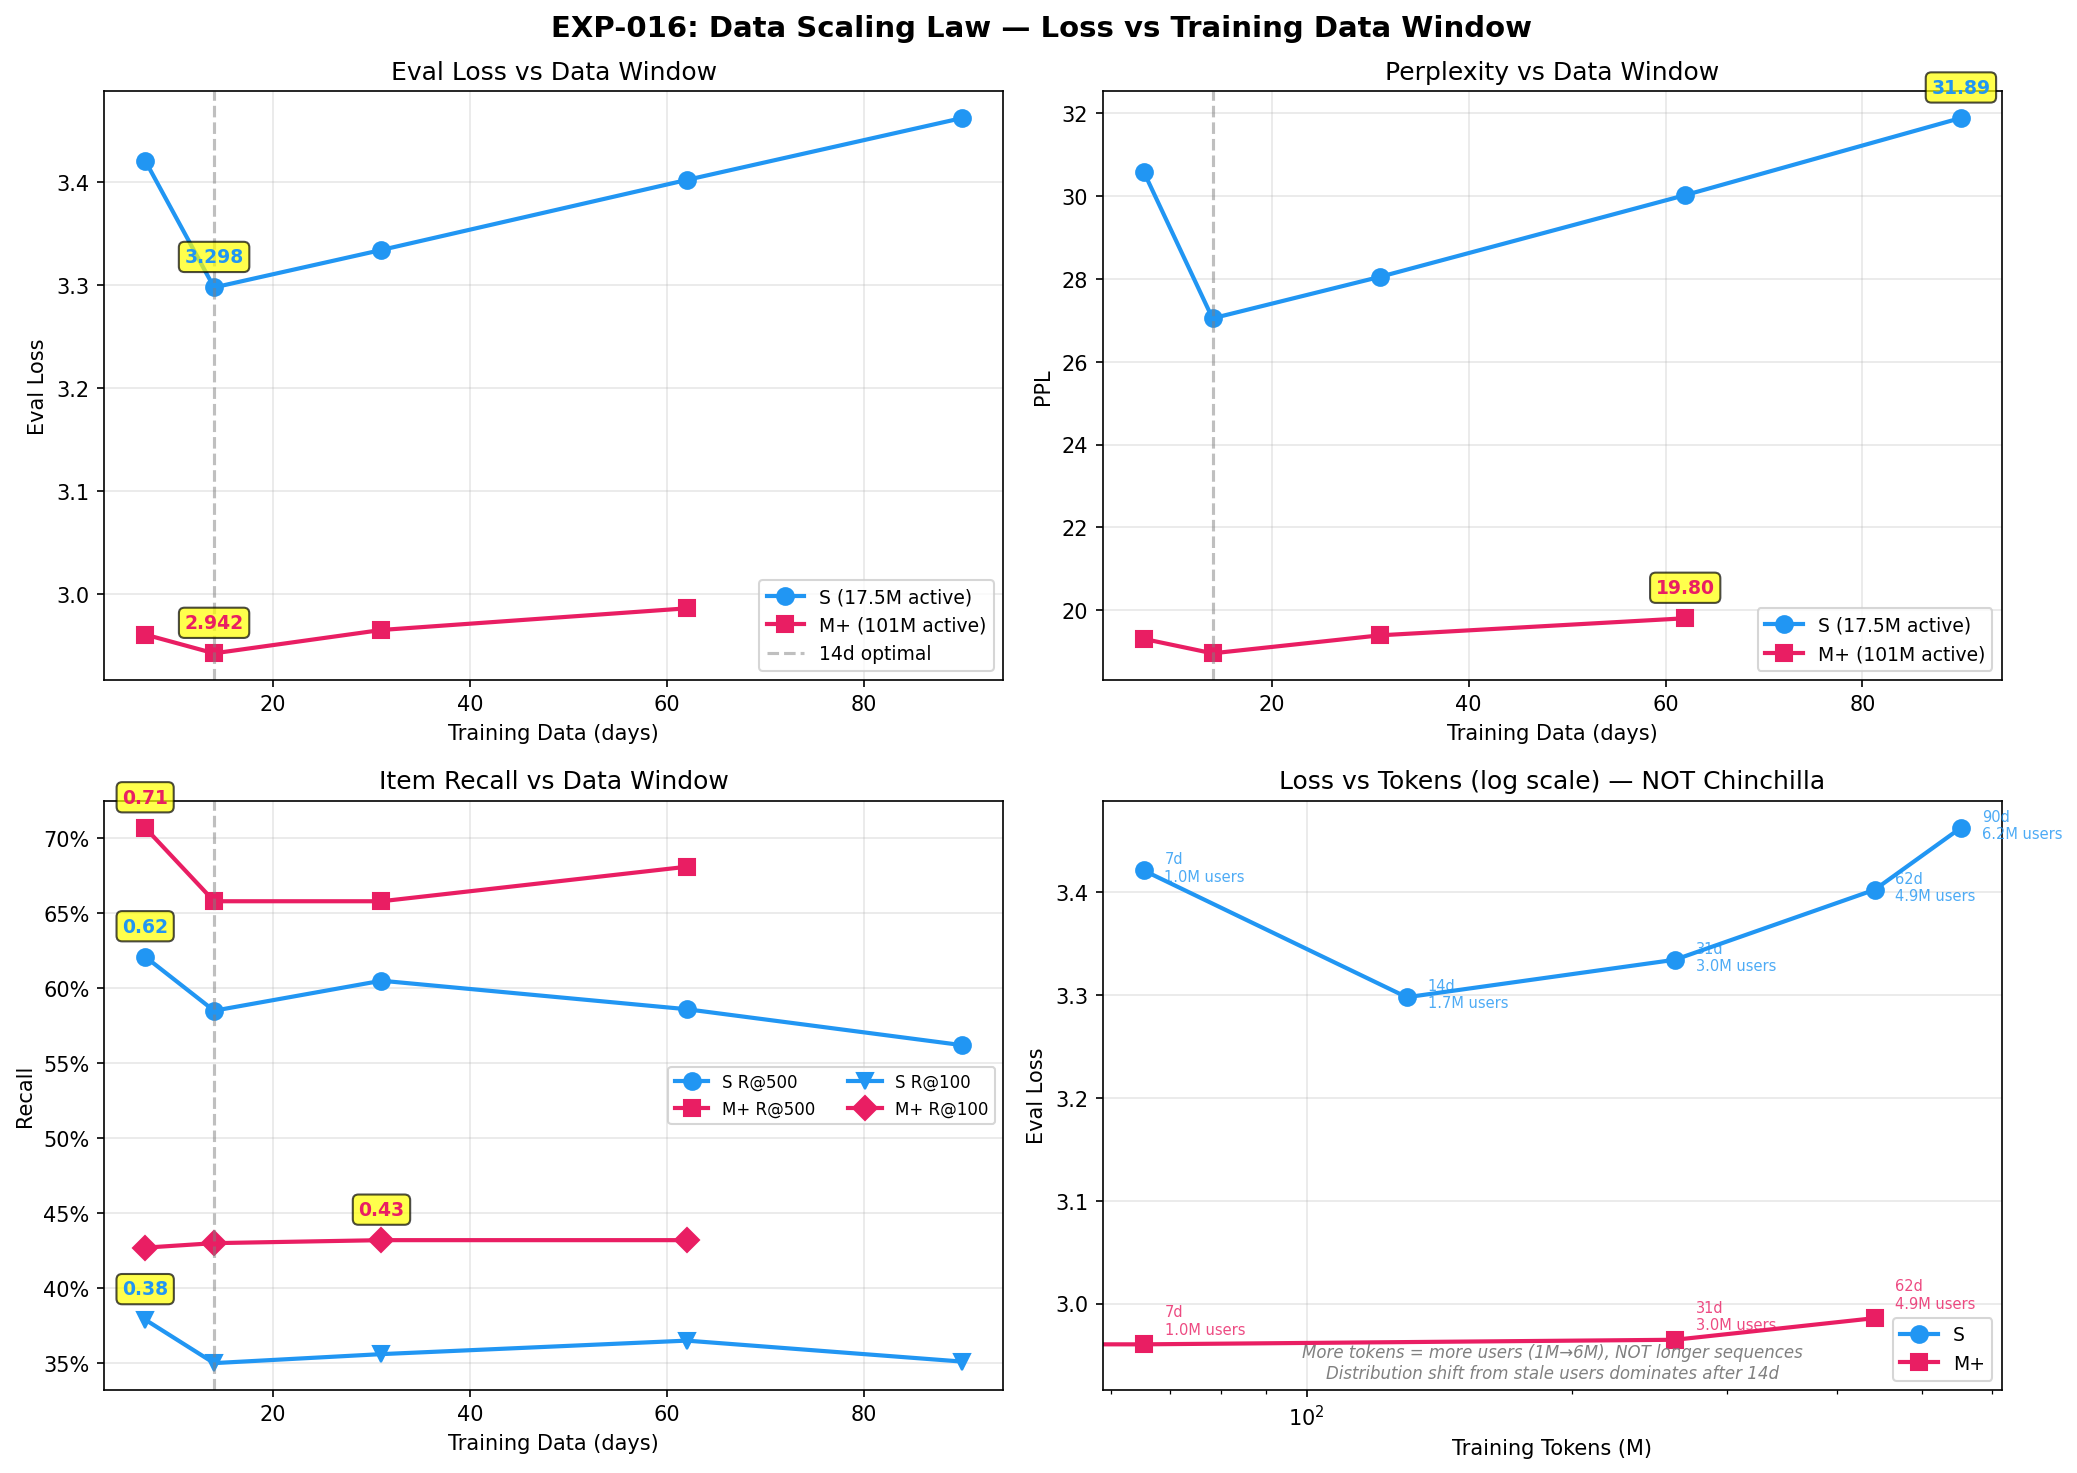
\includegraphics[width=0.78\linewidth]{figures/exp016-data-scaling.png}
\caption{Behavior-window scaling under production temporal drift.}
\label{fig:data-scaling}
\end{figure}

\subsection{Tokenizer and Embedding Sweep}

The third validation target is item representation. Tokenizer quality affects the irreducible loss floor and the search space exposed to beam decoding. We evaluated 14 tokenizer variants over 0.6B and 4B embeddings, uniform 4096/8192 codebooks, MGMR-style hierarchical codebooks, and FSQ hidden sizes. The production SID caches used by the embedding-size comparison cover about 1.10M items (1,096,364--1,110,697 items across 0.6B/4B/8B caches), making the tokenizer metrics item-space rather than toy-codebook measurements. Table~\ref{tab:tokenizer} shows representative results.

\begin{table}[t]
\centering
\caption{Representative tokenizer sweep results. CR is collision rate and snHR is behavior-aware semantic neighbor hit rate.}
\label{tab:tokenizer}
\begin{tabular}{lrrrr}
\toprule
SID Cache & CR & Gini-d1 & Gini-d2 & snHR \\
\midrule
0.6B nc4096 h64 & 0.67\% & 0.3243 & 0.3546 & 0.0797 \\
0.6B nc8192 h128 & 0.42\% & 0.3914 & 0.2375 & 0.0919 \\
4B nc4096 h128 & 1.60\% & 0.2877 & 0.3539 & 0.1255 \\
4B nc8192 h128 & 1.28\% & 0.3192 & 0.2530 & 0.1307 \\
4B nc8192x2048 h128 & 1.41\% & 0.3191 & 0.3170 & 0.1154 \\
\bottomrule
\end{tabular}
\end{table}

The decisive variable in this sweep is the 8192 codebook setting, which improves L2 balance and snHR. The 4B embedding improves semantic-neighbor retention, but also requires enough FSQ capacity to avoid L2 entropy collapse. The current recommended caches are listed in the released experiment logs.

\subsection{Full-Recall Baselines}

The fourth validation target is the full GR retrieval loop. Table~\ref{tab:full-eval} reports current full-eval baselines produced by SID-constrained generation. The strongest observed NTP result is the M-tier model with 4B SID, reaching R@500=70.4\% and R@10=14.2\%. Its train metadata records 1,719,646 training sequences, 134.0M training tokens, 49,159 evaluation items, and 1,000 full-recall samples.

\begin{table}[t]
\centering
\caption{Current full-eval baselines.}
\label{tab:full-eval}
\begin{tabular}{lrrr}
\toprule
Config & R@10 & R@500 & PPL \\
\midrule
S-tier bare & 11.4\% & 61.2\% & 26.52 \\
S-tier with TO-RoPE ts=0.5 & 11.8\% & 63.9\% & 22.7 \\
M-tier bare, 0.6B SID & 14.5\% & 70.2\% & 18.54 \\
M-tier, 4B SID & 14.2\% & 70.4\% & 16.55 \\
L-tier with validated options & 12.8\% & 64.1\% & 20.7 \\
\bottomrule
\end{tabular}
\end{table}

\subsection{Public Execution Proof}

The private production data cannot be redistributed, so the repository includes a separate public MovieLens path. This path is deliberately small and should not be read as a leaderboard benchmark. Its purpose is to prove that the released code can execute the same framework loop on public data and widely available free-GPU infrastructure. The checked-in Colab-T4 run uses 5,950 users, 3,532 items, 348,363 NTP training examples, 348,363 alignment examples, Qwen3 item embeddings, residual KMeans SIDs with a 64$\times$64$\times$64 token space, a dense 3-layer NTP model, 100 lightweight GRPO-style alignment steps, and SID-constrained beam search. The important result is run completeness: the public artifact traverses item metadata $\rightarrow$ Qwen embedding $\rightarrow$ SID construction $\rightarrow$ NTP training $\rightarrow$ reward alignment $\rightarrow$ constrained full-recall evaluation without access to private data.

\subsection{Post-Training Alignment}

The final validation target is post-training. We evaluated preference and RL-style alignment methods, including SP-DPO, RF-DPO, GRPO, and ECPO. The most instructive result is the off-policy/on-policy ECPO comparison in Table~\ref{tab:alignment}. Both ECPO runs use the same 14-day feature shard with 1,709,380 training sequences and 49,456 evaluation targets; the full evaluation samples 1,000 targets from 26,450 evaluation items.

\begin{table}[t]
\centering
\caption{On-policy candidate generation recovers an ECPO collapse.}
\label{tab:alignment}
\begin{tabular}{lrrrr}
\toprule
Config & R@10 & R@500 & PPL & Clip Rate \\
\midrule
Off-policy ECPO & 0.7\% & 2.0\% & 3791 & 99\% \\
On-policy ECPO & 13.0\% & 67.8\% & 14.1 & 92\% \\
SFT baseline & 14.1\% & 66.2\% & 16.3 & -- \\
\bottomrule
\end{tabular}
\end{table}

The off-policy run generates candidates from a reference model whose distribution drifts away from the current policy. This distorts the importance ratio and causes clipping to dominate. On-policy beam candidates better match the current policy distribution, recovering both PPL and R@500. Figure~\ref{fig:alignment} shows the post-training curves.

\begin{figure}[t]
\centering
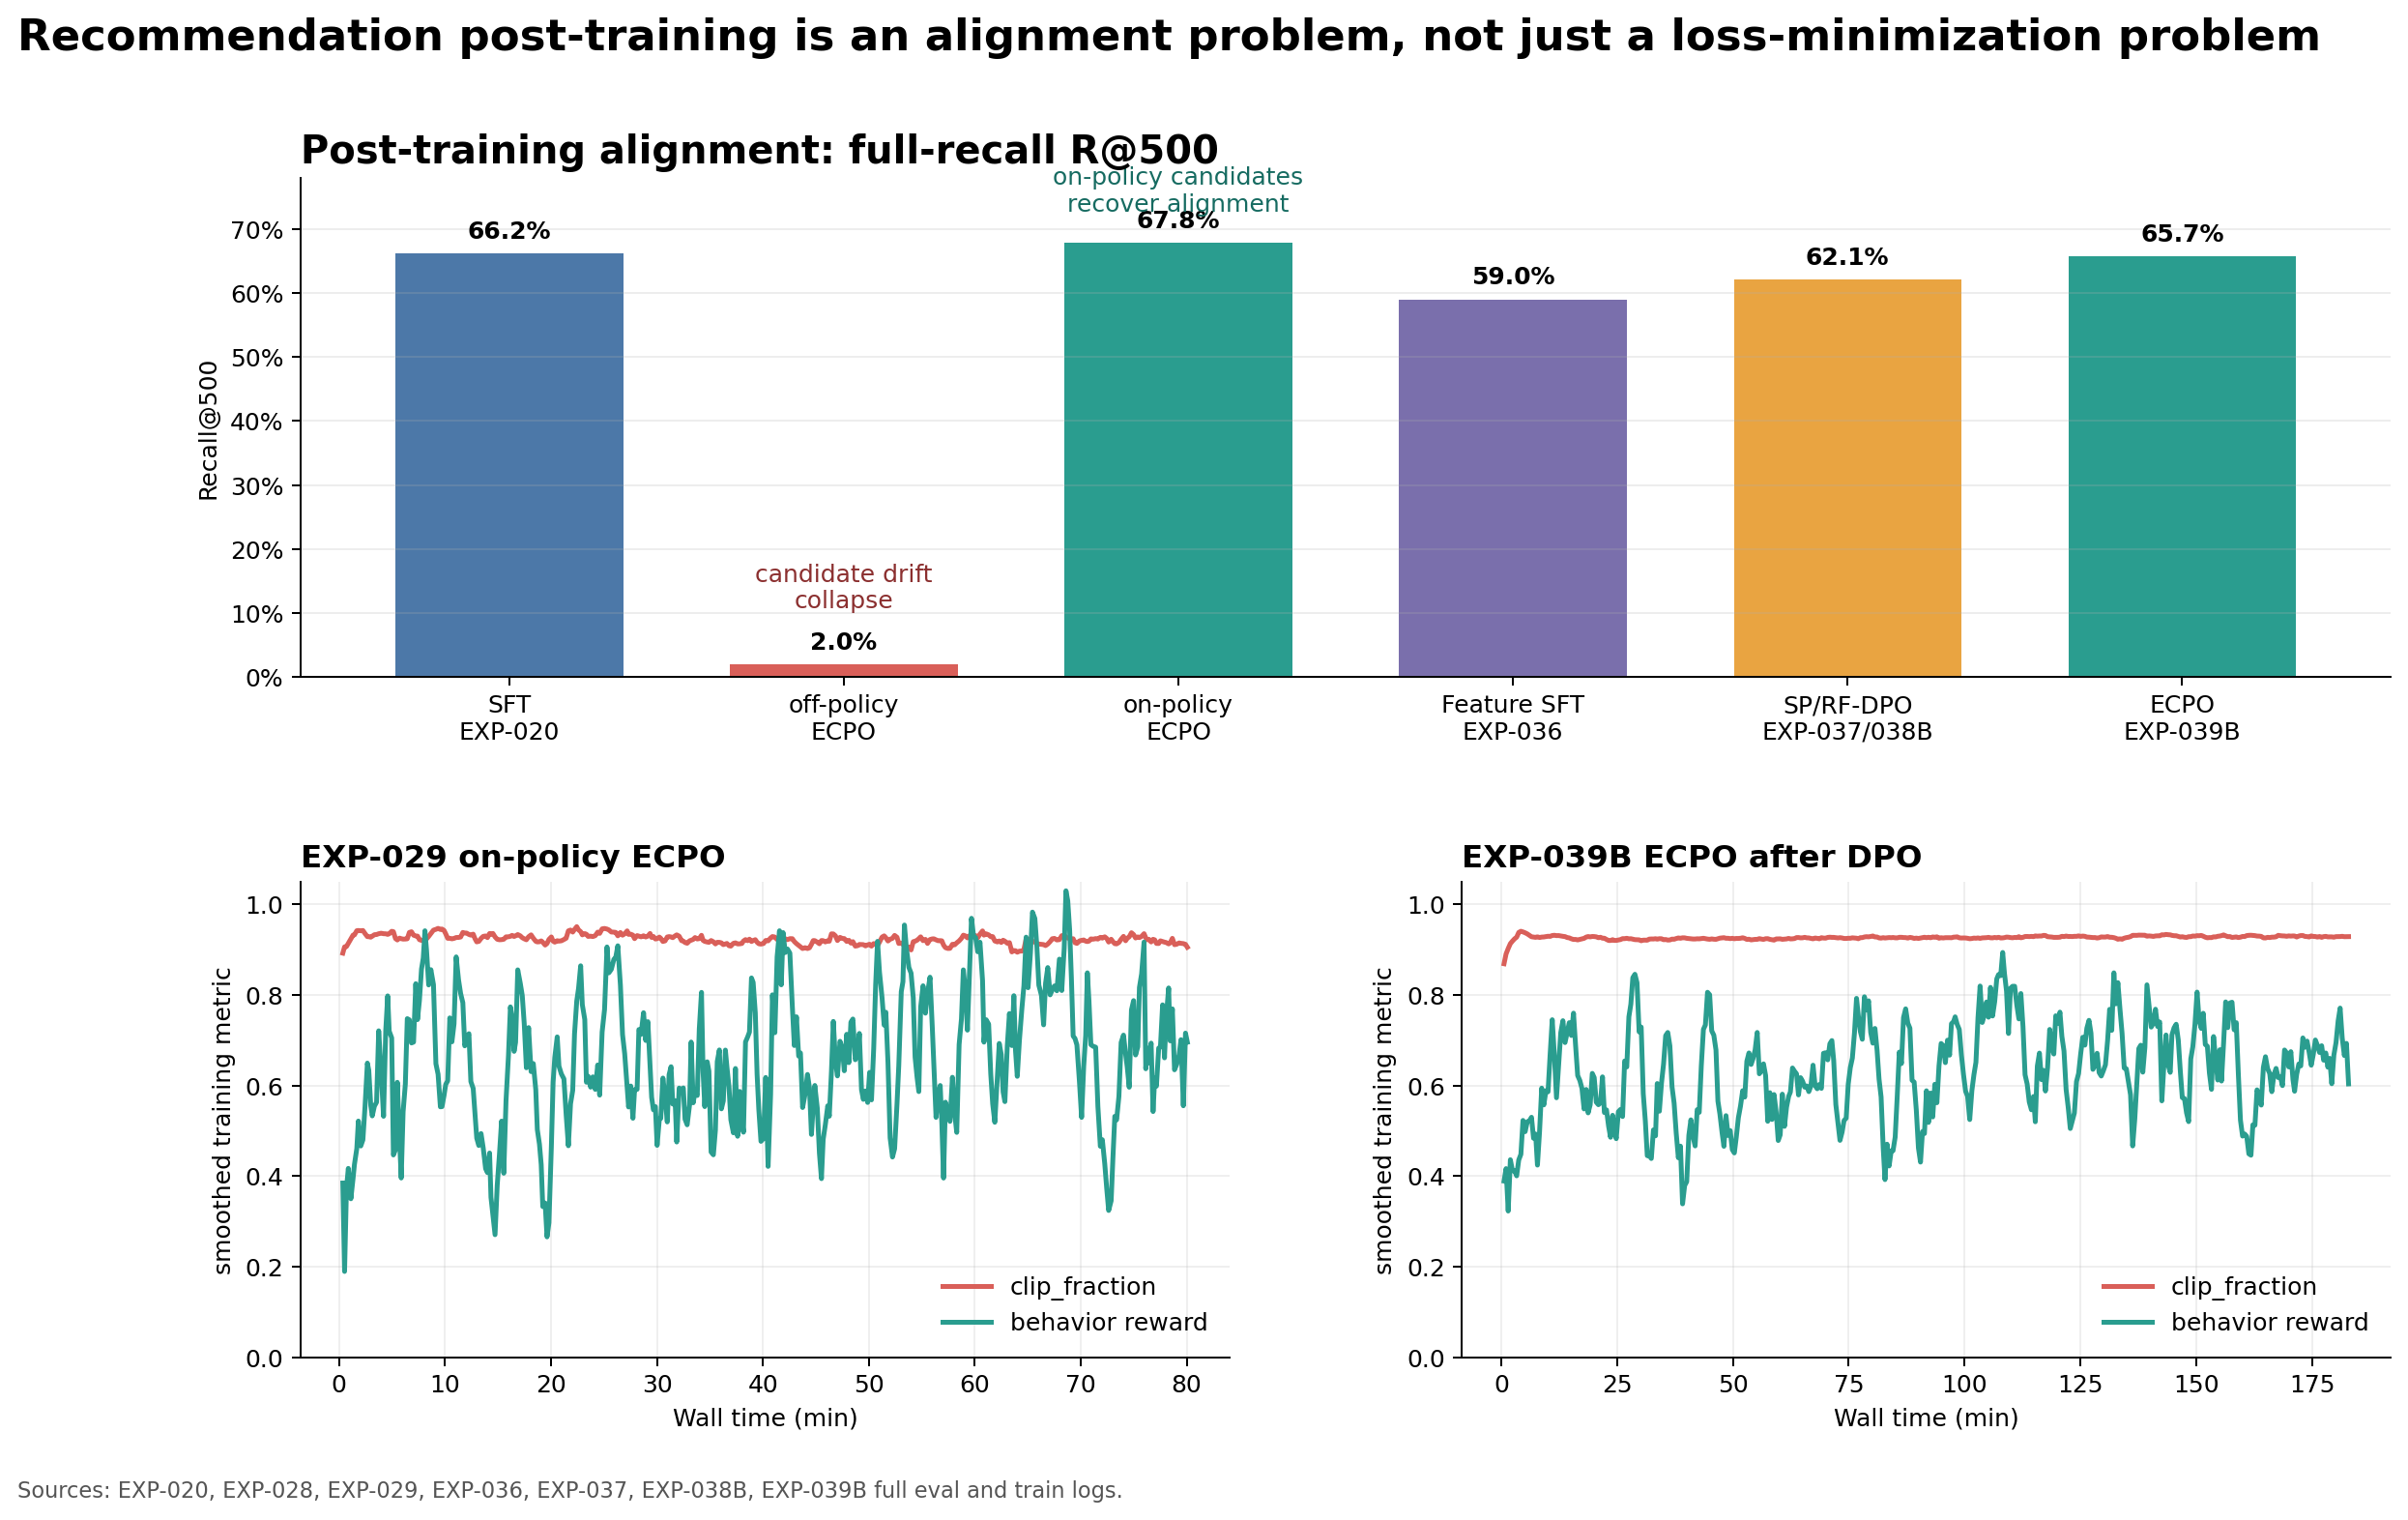
\includegraphics[width=0.78\linewidth]{figures/post_training_alignment.png}
\caption{Post-training alignment curves and collapse/recovery behavior.}
\label{fig:alignment}
\end{figure}

\section{Discussion}

\subsection{Why the Agentic Layer Matters}

The private lineage suggests that the agentic layer is valuable because it shortens the distance between an idea and a trustworthy conclusion. In a conventional workflow, code changes, experiment launch commands, queue state, failed logs, and paper notes often live in separate tools. This separation is tolerable for a single run, but it becomes brittle when a research direction needs dozens of iterations and when GPU jobs continue after the interactive coding session has ended. \textsc{nanoGenRec} keeps these objects in one repository-level state machine. A new idea is converted into a YAML diff, compared against historical configs, launched through a queue, evaluated with a full-recall contract, and then summarized into phase-level records.

This organization also changes how agents can be used. The useful unit is not a single autonomous agent that claims to finish research end to end. The useful unit is a shared research workspace where agents can take different roles over time: one session may implement a tokenizer change, another may monitor long jobs, a later session may inspect logs and write the paper. The explicit inbox/outbox protocol was one implementation of this handoff when coding and experiment agents were separated for operational reasons. Once all agents share the same repository state, the same pattern can be implemented by forked sessions or other task-routing mechanisms. The durable artifacts remain the core interface.

\subsection{What the Framework Makes Reproducible}

The production data cannot be released. However, the artifact makes the following components inspectable and reusable:

\begin{itemize}
  \item model and tokenizer implementations;
  \item preprocessing and evaluation interfaces;
  \item compact public MovieLens paths for checking that the released loop executes without private data;
  \item experiment configs and resolved parameter sets;
  \item full-recall evaluation protocol;
  \item experiment logs with hypotheses, designs, results, and post-hoc analysis;
  \item known invalid runs and bug records.
\end{itemize}

This distinction matters. A GR framework can be useful even when a production dataset is not public, provided that the code path, configuration semantics, evaluation protocol, and empirical record are exposed. The public MovieLens paths demonstrate execution of the loop, but the main reproducibility target of \textsc{nanoGenRec} is the working research process: how to construct SIDs, train the model, align it with reward signals, decode valid items, evaluate full recall, organize experiments, and diagnose failures.

\subsection{Lessons}

Three lessons recur across the experiment lineage. First, landing GR requires full evaluation to be separated from training-time health checks. Second, feature ablations require end-to-end validation across preprocessing, training, and inference; otherwise, experiments can silently compare zeros. Third, post-training alignment in GR is sensitive to candidate distribution, so rollout generation should be treated as part of the algorithm rather than a fixed data-preparation step. These lessons are as much about framework design as model design: most failures arise at component boundaries.

\section{Limitations}

This report has several limitations. The production behavior data is not released, so external users cannot exactly reproduce the reported production-scale numbers. The repository includes MovieLens CPU and Colab-T4 public paths to verify the released framework loop, but these are execution checks rather than competitive public leaderboard claims. The public GRPO-style stage is intentionally lightweight, and its high clip fraction indicates that alignment hyperparameters remain a tuning target rather than a final recipe. The framework currently focuses on Semantic-ID autoregressive recommendation rather than all forms of generative retrieval. Online serving, latency, and deployment integration details are not released. Some post-training methods are preliminary and should be interpreted as framework-validated engineering evidence rather than final algorithmic conclusions. Broader public benchmarking across redistributable datasets would strengthen external empirical validation, while the current contribution remains the agentic framework and production-grounded research record.

\section{Conclusion}

We presented \textsc{nanoGenRec}, an open-source agentic research framework for landing Semantic-ID generative recommendation. The project contributes a human-agent research protocol, experiment orchestration system, end-to-end GR workflow, full-recall evaluation contract, and 51-experiment lineage from a real business research setting. Within this framework, we reproduce several valuable GR outputs: model scaling, non-monotonic behavior-window scaling, tokenizer and embedding effects, full-recall baselines, and post-training alignment collapse/recovery. The central result is not a new standalone algorithm, but a working, inspectable research loop from paper reading and hypothesis formation to Semantic-ID construction, real-item generative retrieval, evaluation, logging, and failure-aware iteration. We hope the artifact helps researchers, practitioners, and research agents turn Generative Recommendation from a collection of system diagrams into an extensible, production-grounded research workflow.

\paragraph{Artifact.}
The code and experiment logs are available in the public nanoGenRec repository.\footnote{\url{https://github.com/yzq986/nanoGenRec}}

\bibliographystyle{plainnat}
\bibliography{references}

\end{document}
